\documentclass[12pt, letterpaper] {article}

\parindent=5mm
\usepackage[spanish]{babel}

\usepackage{amssymb}
\usepackage{amsmath} 
\usepackage{amsfonts}

\usepackage[numbers,sort&compress]{natbib}
\usepackage{graphicx}

\usepackage{url}
\usepackage{hyperref}

\usepackage[top=25mm, bottom=20mm, left=1.5cm, right=1.5cm]{geometry}
\setlength{\parskip}{2mm}
\setlength{\parindent}{1pt}

\usepackage{listings}

\usepackage{float}

\usepackage[utf8]{inputenc}
\usepackage{graphicx} 
\usepackage{subfigure} 

\usepackage{color}
\usepackage{multirow}

\definecolor{dkgreen}{rgb}{0,0.6,0}
\definecolor{gray}{rgb}{0.5,0.5,0.5}
\definecolor{mauve}{rgb}{0.58,0,0.82}

\usepackage{color}
\usepackage{listings}
\lstset{ %
  language=R,                     % the language of the code
  basicstyle=\footnotesize,       % the size of the fonts that are used for the code
  numbers=left,                   % where to put the line-numbers
  numberstyle=\tiny\color{gray},  % the style that is used for the line-numbers
  stepnumber=1,                   % the step between two line-numbers. If it's 1, each line
                                  % will be numbered
  numbersep=5pt,                  % how far the line-numbers are from the code
  backgroundcolor=\color{white},  % choose the background color. You must add \usepackage{color}
  showspaces=false,               % show spaces adding particular underscores
  showstringspaces=false,         % underline spaces within strings
  showtabs=false,                 % show tabs within strings adding particular underscores
  frame=single,                   % adds a frame around the code
  rulecolor=\color{black},        % if not set, the frame-color may be changed on line-breaks within not-black text (e.g. commens (green here))
  tabsize=2,                      % sets default tabsize to 2 spaces
  captionpos=b,                   % sets the caption-position to bottom
  breaklines=true,                % sets automatic line breaking
  breakatwhitespace=false,        % sets if automatic breaks should only happen at whitespace
  title=\lstname,                 % show the filename of files included with \lstinputlisting;
                                  % also try caption instead of title
  keywordstyle=\color{blue},      % keyword style
  commentstyle=\color{dkgreen},   % comment style
  stringstyle=\color{mauve},      % string literal style
  escapeinside={\%*}{*)},         % if you want to add a comment within your code
  morekeywords={*,...}            % if you want to add more keywords to the set
} 

\usepackage{booktabs}
\usepackage[table,xcdraw]{xcolor}


\author{Ricardo Rosas Macías}

\title{Práctica 4: diagramas de Voronoi}

\date{\today}

\begin{document}

\maketitle



\section{Introducción}

Los diagramas de Voronoi \cite{articlevoronoi} o también conocidos como polígonos de Thiessen, son una observación básica en la Geometría Computacional, estos son un agregado de puntos en un plano, que tiene una región delimitada por el tamaño de los vecinos; por ende cada punto almacena toda la información acorde a la cercanía entre los demás puntos de su alrededor.

 \section{Objetivo}

El objetivo principal de la práctica es determinar el comportamiento de la grieta respecto a la variación de los parámetros que generan la Teselación de Voronoi, asimismo examinar de una manera cuantitativa la varianza de los factores que alteran el tamaño de la grieta.

 \subsection{Descripción}

Lo que se debe hacer es \cite{elisawebDV}:
\begin{quotation}
 ``Examinar de manera sistemática el efecto del número de semillas y del tamaño de la zona en la distribución de los largos de las grietas que se forman con dos medidas para el largo de una grieta: el número de celdas que contiene la grieta y la mayor distancia Manhattan entre la grieta y el borde del cuadro.''
\end{quotation}

\section{Resultados y conclusiones}

Para llevar acabo el experimento se realizó cambios en el código \cite{EMP4} con ayuda de la literatura \cite{P4As}. En las líneas de código que se muestran debajo, en donde el acomodo de las semillas se realizó de manera aleatoria en conjuntos de 10 -- 50 en intervalos de 10, de la misma manera la cuadricula se ejecutó en 50 -- 300 en intervalos de 50. En la parte inferior se plantea la ejecución de un análisis de varianza; de este modo proporcionó el comportamiento que tiene la grieta al realizar cambios en las variables. Además se hizo un Gif para tener una visualización del cambio del tamaño de la grieta.

\begin{lstlisting}[language=R]
suppressMessages(library(doParallel))
registerDoParallel(makeCluster(detectCores() - 1))
Manhattan <- TRUE
N <- c(50, 300, 50)
K <- c(10, 50, 10)
Info <- data.frame()
Largo <- c()
Nys <- c()
Kys <- c()
for (n in N) {
  for (k in K){
    zona <- matrix(rep(0, n * n), nrow = n, ncol = n)
    x <- rep(0, k) 
    y <- rep(0, k) 
    
    for (semilla in 1:k) {
      while (TRUE) { 
        fila <- sample(1:n, 1)
        columna <- sample(1:n, 1)
        if (zona[fila, columna] == 0) {
          zona[fila, columna] = semilla
          x[semilla] <- columna
          y[semilla] <- fila
          break
        }
      }
    }
    celdas <- foreach(p = 1:(n * n), .combine=c) %dopar% celda(p)
    stopImplicitCluster()
    voronoi <- matrix(celdas, nrow = n, ncol = n, byrow=TRUE)
    rotate <- function(x) t(apply(x, 2, rev))    
    Lmin <- n 
    vp <- data.frame(numeric(), numeric()) 
    for (dx in -1:1) {
      for (dy in -1:1) {
        if (dx != 0 | dy != 0) { 
          vp <- rbind(vp, c(dx, dy))
        }
      }
    }
    names(vp) <- c("dx", "dy")
    vc <- dim(vp)[1]
    
    registerDoParallel(makeCluster(detectCores() - 1))
    largos <- foreach(r = 1:200, .combine=c) %dopar% propaga(r)
    stopImplicitCluster()
    Sum <- c(n, k, summary(largos))
    Info <- rbind(Info, Sum)
    Largo <- c(Largo, largos)
    Nys <- c(Nys, rep(n, 200))
    Kys <- c(Kys, rep(k, 200))
    colnames(Info) <- c("n", "k", "Min", "Q1", "Median", "Mean", "Q3", "Max")
  }
}
Nys <- factor(Nys)
Kys <- factor(Kys)
summary(aov(Largo ~ Nys * Kys))
system("convert -delay 50 -size 300x300 p4g_*.png -loop 0 Voronoi.gif") 
\end{lstlisting}\vspace{-2mm}

Con la ejecución del código se obtuvo la Teselación de Voronoi que es mostrada en la figura \ref{PI}, en la cual se puede observar la posición inicial de las semillas. Asimismo se hicieron diagramas de Voronoi con la grieta en ellos, se tomó los mas representativos que son mostrados en la figura \ref{G1}, \ref{G2} y \ref{G3}.

\begin{figure}[H]
\centering
\subfigure[]{\includegraphics[width=61mm]{./p4g_0} \label{PI}}\vspace{-1mm}
\subfigure[]{\includegraphics[width=61mm]{./p4g_24} \label{G1}}\vspace{-1mm}\\
\subfigure[]{\includegraphics[width=61mm]{./p4g_29} \label{G2}}\vspace{-1mm}
\subfigure[]{\includegraphics[width=61mm]{./p4g_195} \label{G3}}\vspace{-1mm}
\caption{Diagramas de Voronoi del experimento} \label{DVF}
\end{figure}

En la figura \ref{LGr} y \ref{DMan} se aprecia la afinidad de disminución en las zonas con un mayor tamaño. Por lo que la variación de los datos repercuten significativamente en el largo de la grieta final. Por consiguiente se puede observar un decremento en la distancia manhattan y grieta al tener una cuadricula de 50 en relación al tamaño de la zona en comparación con las demás cuadriculas que en muestran una afinidad normal entre la grieta y el borde del cuadro.

\begin{figure}[H]
\centering
\subfigure[Tamaño de grieta]{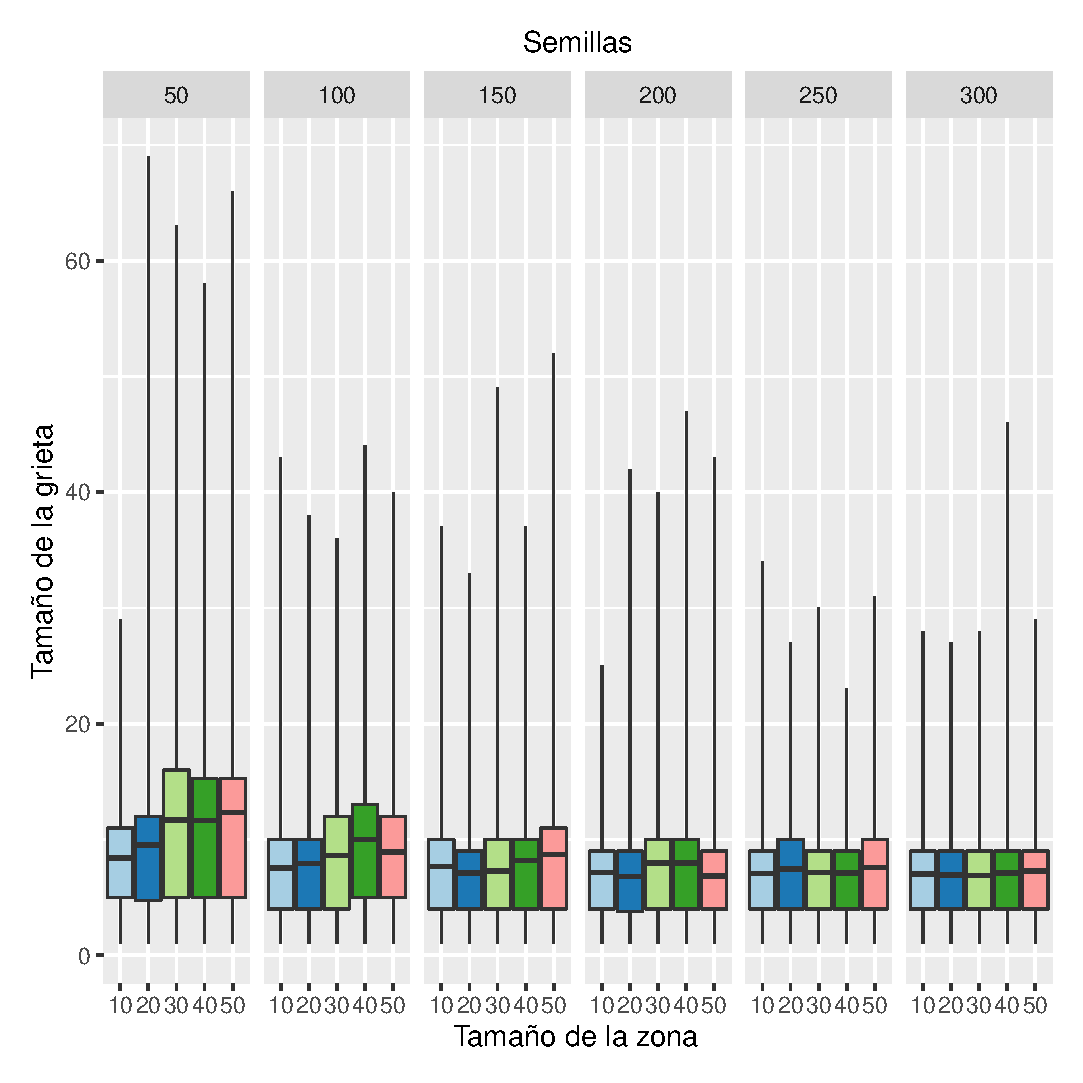
\includegraphics[width=85mm]{./DManh} \label{DMan}}\vspace{-1mm}
\subfigure[Distancia Manhattan]{\includegraphics[width=85mm]{./Tgrieta} \label{LGr}}\vspace{-1mm}
\caption{Resultados de ejecución del experimento} \label{DMTG}
\end{figure}\vspace{-2mm}

Por último, como se menciono anteriormente, se realizó un análisis ANOVA factorial que permitió determinar la varianza del tamaño de la grieta de acuerdo a su distancia Manhattan y semillas usadas, estos datos son mostrados en el cuadro \ref{datab}. En el que se puede observar que se tiene un nivel debajo del 0.05 en $Pr(>F)$, de modo que ocasiona una ligera diferencia en las medias, que muestran una diferencia significativa en el crecimiento de las grietas respecto a la disminución de las semillas.\vspace{-3mm}

\begin{table}[H]
\centering
\caption{Comparación de tiempo de ejecución, normal versus paralelizada.}
\label{datab}
\begin{tabular}{@{}|l|l|l|l|l|l|@{}}
\hline
\rowcolor[HTML]{ECF4FF} 
\multicolumn{1}{|c|}{\cellcolor[HTML]{ECF4FF}{\color[HTML]{333333} }} & {\color[HTML]{333333} Gl}    & {\color[HTML]{333333} Suma Cuad.} & {\color[HTML]{333333} Media Cuad.} & {\color[HTML]{333333} Valor F} & {\color[HTML]{333333} Pr(\textgreater{}F)} \\ \hline
\rowcolor[HTML]{EFEFEF} 
{\color[HTML]{333333} Tamaño de zona}                                 & {\color[HTML]{333333} 5}    & {\color[HTML]{333333} 9580}       & {\color[HTML]{333333} 1916.1}      & {\color[HTML]{333333} 52.523}  & {\color[HTML]{333333} \textless 2e-16}     \\ \hline
\rowcolor[HTML]{EFEFEF} 
{\color[HTML]{333333} Semillas}                                       & {\color[HTML]{333333} 4}    & {\color[HTML]{333333} 1481}       & {\color[HTML]{333333} 370.2}       & {\color[HTML]{333333} 10.149}  & {\color[HTML]{333333} 3.47e-08}            \\ \hline
\rowcolor[HTML]{EFEFEF} 
{\color[HTML]{333333} Tamaño Zona vs Semillas}                        & {\color[HTML]{333333} 20}   & {\color[HTML]{333333} 2155}       & {\color[HTML]{333333} 107.8}       & {\color[HTML]{333333} 2.954}   & {\color[HTML]{333333} 1.06e-05}            \\ \hline
\rowcolor[HTML]{EFEFEF} 
{\color[HTML]{333333} Residuales}                                     & {\color[HTML]{333333} 5970} & {\color[HTML]{333333} 217792}     & {\color[HTML]{333333} 36.5}        & {\color[HTML]{333333} }        & {\color[HTML]{333333} }                    \\ \hline
\end{tabular}
\end{table}\vspace{-10mm}



\bibliographystyle{plainnat}

\bibliography{BHWP4}


\end{document} 